\documentclass[11pt]{article}

\usepackage[margin=1in]{geometry}
\usepackage{amsmath,amssymb}
\usepackage{booktabs}
\usepackage{graphicx}
\usepackage[hidelinks]{hyperref}

\title{\vspace{-1.2cm}Spherical Decision Trees: A Short Geometric Note}
\author{Mathias Valla}
\date{\today}

\begin{document}
\maketitle

\begin{abstract}
Classical decision trees split the covariate space with coordinate thresholds.
This rectangular geometry is simple and effective, but it can be inefficient
when the response is controlled by a localized region of the feature space, for
example observations close to a prototype, a centroid, or a compact cluster. We
study a small modification of recursive partitioning in which a node sends
observations left or right according to whether they fall inside or outside a
hypersphere. The method keeps the familiar tree architecture while replacing
some one-dimensional threshold questions by distance-to-center questions. We
describe the construction, give a simple geometric argument showing that distant
sphere centers recover linear splits as a local limiting case, and summarize an
exploratory benchmark against axis-aligned and oblique trees. The results
suggest that spherical forests can be competitive for classification problems,
while single spherical trees and regression settings remain more fragile. We
therefore view spherical splits not as a replacement for CART, but as a
complementary local geometry for tree-based models.
\end{abstract}

\section{Motivation}

Decision trees are attractive because they are nonparametric, interpretable, and
easy to ensemble. Their usual form, however, is tied to a strong geometric
choice. At each internal node, CART-style trees select a feature index $j$ and a
threshold $a$, then split observations according to $x_j \le a$ or $x_j>a$
\cite{breiman1984cart}. Recursively, this produces rectangular cells.

Rectangular cells are natural when the signal is sparse and coordinate-aligned.
They are less economical when the target depends on an area around a center. In
classification, a class may correspond to a compact region; in regression, a
response surface may change around a point, centroid, or prototype. An
axis-aligned tree can approximate such a region, but it may need many cuts. A
spherical split can isolate the same region directly.

\section{Spherical splits}

Let $S\subseteq\{1,\ldots,p\}$ be the set of features used at a node. A
spherical split is defined by a center $c\in\mathbb{R}^{|S|}$ and a radius
$r\ge 0$:
\[
    \|x_S-c\|_2^2 \le r^2.
\]
Observations satisfying this inequality are sent to one child and the remaining
observations to the other child. The pair $(c,r)$ is selected to maximize the
same impurity decrease used in ordinary tree induction, such as Gini decrease
for classification or variance reduction for regression.

In the implementation studied here, candidate centers are generated from a
finite mixture of rules: global centers, target-conditional centers, observed
points, pairwise midpoints, local Gaussian perturbations, and farther radial
perturbations. For each candidate center, candidate radii are induced by the
Euclidean distances from the center to node samples. This preserves the usual
finite split search structure: the geometry changes, but the recursive
optimization problem remains a sequence of impurity comparisons.

Figure~\ref{fig:geometry} shows a two-dimensional example. The learned rule at
each internal node is a circle; the terminal regions arise from recursive
inside/outside decisions.

\begin{figure}[t]
    \centering
    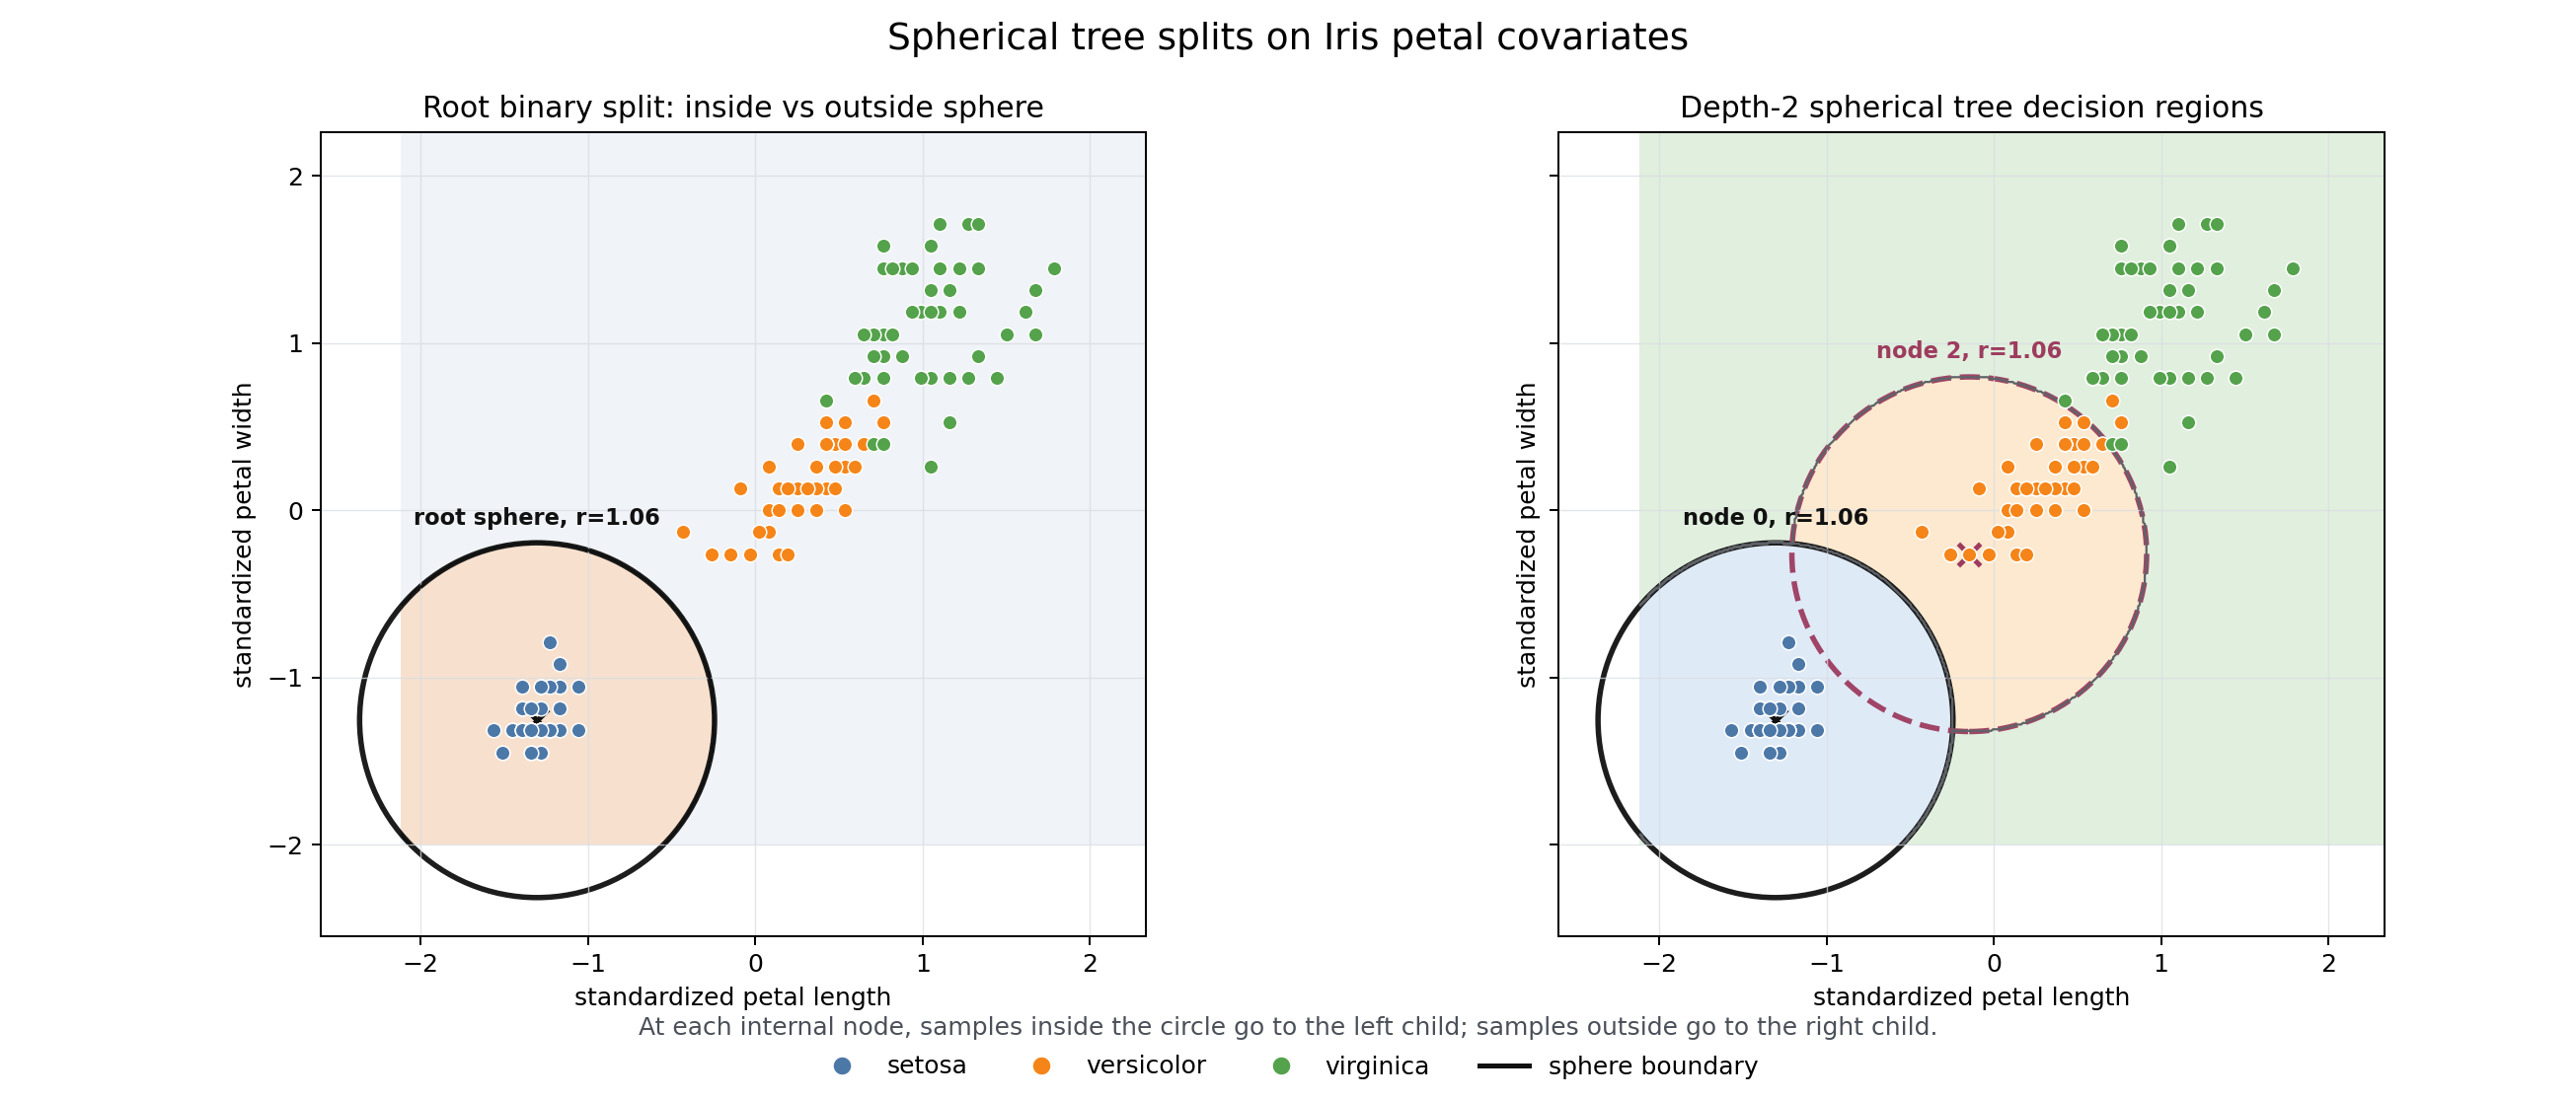
\includegraphics[width=0.92\linewidth]{figures/geometry_iris_partition.png}
    \caption{A two-dimensional spherical decision tree on Iris features. Each
    circle is a learned split frontier; samples inside the circle go to one
    child, and samples outside go to the other child.}
    \label{fig:geometry}
\end{figure}

\section{Two useful geometric facts}

The first useful case is local radial structure. If the target changes when
$x$ enters a ball around $c$, then a single spherical split can represent that
event. A rectangular tree, by contrast, must approximate the ball by many
coordinate cuts. This is an approximation-economy argument rather than a claim
that spherical trees are universally more expressive.

The second useful case is the limiting connection to linear splits. Let
$u\in\mathbb{R}^p$ satisfy $\|u\|_2=1$, let $R>0$, set $c=Ru$, and choose
\[
    r_R^2 = R^2 - 2Rt.
\]
Then
\[
\begin{aligned}
    \|x-Ru\|_2^2 \le r_R^2
    &\Longleftrightarrow
    \|x\|_2^2 - 2R u^\top x + R^2 \le R^2 - 2Rt \\
    &\Longleftrightarrow
    u^\top x \ge t + \frac{\|x\|_2^2}{2R}.
\end{aligned}
\]
On any bounded region $\|x\|_2\le B$, the final term is at most
$B^2/(2R)$. Thus the spherical split converges locally to the halfspace
$u^\top x\ge t$ as the center is moved far away. Axis-aligned splits are
recovered by taking $u$ equal to a coordinate vector. In finite samples this is
only a local approximation, but it motivates center-generation schemes that
include far-away candidates.

\section{Exploratory benchmark}

We implemented spherical trees and spherical random forests in \texttt{treeple}
and compared them with axis-aligned CART and random forests, as well as oblique
trees and forests. The benchmark used complete PMLB datasets that ran without
errors, plus simple two-dimensional toy classification datasets. Features were
imputed and standardized. The main benchmark used three cross-validation folds,
50 trees for forests, 500 spherical center candidates per node, all data-induced
radii for each candidate center, validation-selected pruning for single trees,
and unpruned forests. Large datasets were capped at 1000 sampled observations.
The final comparison contained 249 complete datasets and 38 skipped datasets
or fetch/model errors. The comparison is descriptive: it is intended to
characterize regimes and failure modes, not to prove dominance.

\begin{table}[t]
    \centering
    \caption{Mean benchmark performance and fit time over complete datasets.
    Primary score is balanced accuracy for classification and $R^2$ for
    regression.}
    \label{tab:benchmark}
    \begin{tabular}{llrrr}
        \toprule
        Task & Model & Datasets & Score & Fit time (s)\\
        \midrule
        Classification & Spherical random forest & 132 & 0.765 & 9.850\\
        Classification & Random forest & 132 & 0.738 & 0.137\\
        Classification & Oblique random forest & 132 & 0.737 & 0.154\\
        Classification & CART & 132 & 0.722 & 0.074\\
        Classification & Oblique tree & 132 & 0.706 & 0.136\\
        Classification & Spherical tree & 132 & 0.688 & 4.132\\
        \midrule
        Regression & Random forest & 117 & 0.717 & 0.384\\
        Regression & Oblique random forest & 117 & 0.700 & 0.434\\
        Regression & Spherical random forest & 117 & 0.665 & 20.533\\
        Regression & CART & 117 & 0.521 & 0.078\\
        Regression & Oblique tree & 117 & 0.391 & 0.093\\
        Regression & Spherical tree & 117 & 0.262 & 7.516\\
        \bottomrule
    \end{tabular}
\end{table}

The main pattern is mixed. Spherical random forests perform well on
classification in this run, obtaining the best mean classification score in
Table~\ref{tab:benchmark}, but at a substantial computational cost. For
regression, ordinary and oblique random forests remain stronger. Single
spherical trees are not competitive on average, which suggests that the
spherical geometry is most useful when stabilized by ensembling or when the data
contain very clear radial structure.

Figure~\ref{fig:regime} gives a compact view of the empirical regime map. It
should be read cautiously: the number of rows and predictors alone does not
fully determine when spherical splits help. The missing variable is likely
geometric: whether the target depends on local neighborhoods, clusters, or
distance-to-prototype effects.

\begin{figure}[t]
    \centering
    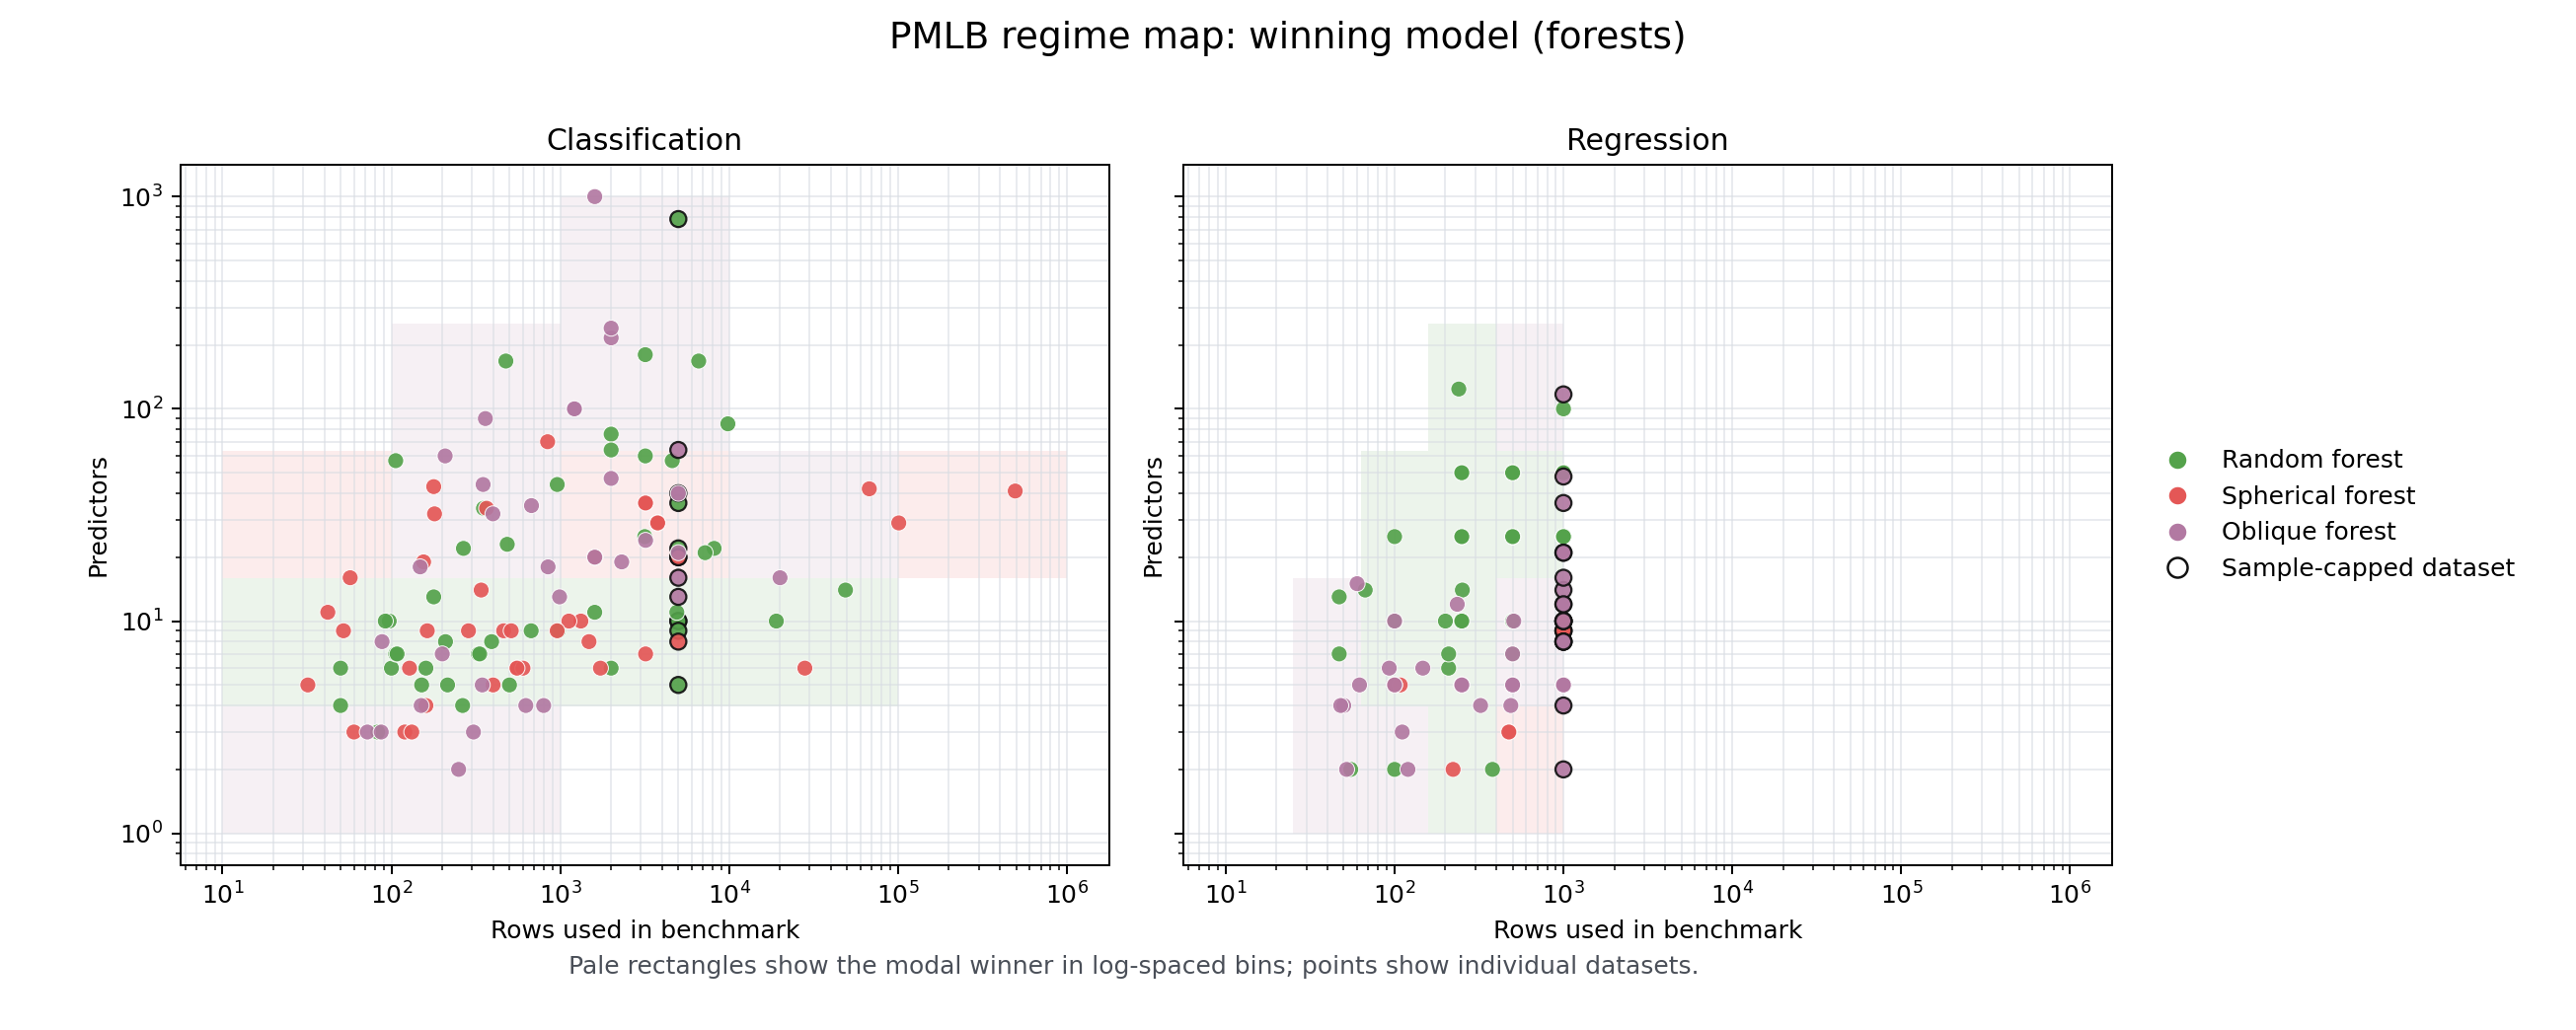
\includegraphics[width=0.92\linewidth]{figures/benchmark_regime_forests.png}
    \caption{Winning forest model across benchmark datasets as a function of
    sample size and feature count. The pattern is exploratory and does not
    provide a deterministic rule, but it suggests that spherical forests are a
    useful complement in some classification regimes.}
    \label{fig:regime}
\end{figure}

\section{Limitations}

Spherical trees introduce several costs. Training is slower because each node
must evaluate multiple candidate centers and radii. If a node contains $n_m$
samples, $s$ active features, and $C$ candidate centers, computing distances is
roughly $O(C n_m s)$ and evaluating sorted candidate radii can add
$O(C n_m\log n_m)$. This is much more expensive than scanning coordinate
thresholds.

The method also depends on the metric. In our experiments, predictors were
standardized before fitting. Without scaling, a spherical split is dominated by
high-variance coordinates. In high-dimensional spaces, Euclidean distances can
become less informative, and far-away centers may make splits nearly linear
without solving the underlying greedy-search problem.

The XOR example is instructive. In principle, two far-away circles can locally
approximate the two axis-aligned cuts needed for XOR. A greedy impurity
criterion, however, may reject those cuts at the root because each individual
axis split has little immediate impurity gain. This does not contradict the
linear-limit argument. It shows that spherical trees inherit the myopia of
ordinary greedy tree induction. A depth-two lookahead or delayed-gain criterion
would be needed to systematically recover such interactions.

\section{Conclusion}

Spherical splits provide a simple geometric extension of recursive
partitioning. They are most appealing when the target is expected to depend on
membership in an area of the covariate space, especially around a center or
prototype. They also include linear frontiers as a local limiting case when
centers are allowed to move far from the data. Empirically, the current
implementation is promising for classification forests but slower and less
stable for single trees and regression.

The natural next step is a hybrid tree that chooses among axis-aligned,
oblique, and spherical split candidates at each node, possibly with a small
lookahead window. Such a model would keep the interpretability of recursive
partitioning while allowing the geometry of each decision to adapt locally.

\paragraph{Journal fit.}
Among the two venues considered, \emph{Annals of Mathematics and Artificial
Intelligence} is the better fit for the present letter because it explicitly
targets mathematical and algorithmic methods for artificial intelligence and
machine learning. \emph{Mathematics} is plausible, but would likely require a
more theorem-driven treatment or a broader mathematical analysis.

\begin{thebibliography}{9}

\bibitem{breiman1984cart}
Breiman, L., Friedman, J. H., Olshen, R. A., and Stone, C. J.
\newblock \emph{Classification and Regression Trees}.
\newblock Wadsworth, 1984.

\bibitem{breiman2001rf}
Breiman, L.
\newblock Random forests.
\newblock \emph{Machine Learning}, 45:5--32, 2001.

\bibitem{murthy1994oc1}
Murthy, S. K., Kasif, S., and Salzberg, S.
\newblock A system for induction of oblique decision trees.
\newblock \emph{Journal of Artificial Intelligence Research}, 2:1--32, 1994.

\bibitem{olson2017pmlb}
Olson, R. S., La Cava, W., Orzechowski, P., Urbanowicz, R. J., and Moore, J. H.
\newblock PMLB: a large benchmark suite for machine learning evaluation and
comparison.
\newblock \emph{BioData Mining}, 10:36, 2017.

\bibitem{pedregosa2011sklearn}
Pedregosa, F. et al.
\newblock Scikit-learn: machine learning in Python.
\newblock \emph{Journal of Machine Learning Research}, 12:2825--2830, 2011.

\end{thebibliography}

\end{document}
